\documentclass[10pt]{article}
\usepackage{polski}
\usepackage[utf8]{inputenc}
\usepackage{graphicx}
\title{Specyfikacja implementacyjna projektu związanego z algorytmami operującymi na grafach}
\author{Adrian Nowosielski\\Cezary Skorupski}
\date{05.05.2022}
\begin{document}
\maketitle
\thispagestyle{empty}
\newpage
\thispagestyle{empty}
\begin{center}
    \textbf{\Large{Streszczenie}}\\
    Dokument specyfikacji implementacyjnej projektu \textbf{Grafy} stanowi opis tematyki oprogramowania pod kątem implementacji rozwiązania. Specyfikacja implementacyjna wyjaśnia takie aspekty programu, jak budowę, sposób przeprowadzania testów i podejście konceptualne przyświecające proces tworzenia programu. Dokument specyfikacji implementacyjnej stanowi źródło wiedzy dla osób zainteresowanych działaniem/budową programu.
\end{center}
\newpage
\newpage
\begin{center}
    \tableofcontents
    \thispagestyle{empty}
\end{center}
\newpage
\pagenumbering{arabic}
\section{Informacje ogólne}
\subsection{Problematyka projektu}
Projekt jest przygotowywany na zajęcia JIMP2 na Politechnice Warszawskiej. Program ma służyć do analizy grafów, które mają specjalną postać-można przedstawić je w postaci siatki, takiej jak papier w kratkę. Skrzyżowania kratek to węzły, a linie pionowe i poziome to krawędzie. Dodatkowo analizowane grafy są ważone, czyli każda krawędź w grafie ma przyporządkowaną jakąś wagę z określonego zakresu. Projekt \textbf{Grafy} daje możliwość uruchomienia działania algorytmów badających najkrótsze ścieżki w grafie oraz algorytmów badających spójność w grafie. W analizowanym programie po wczytaniu przez użytkownika grafu lub wygenerowaniu grafu, wyświetla się on na środku ekranu aplikacji. Węzły w grafie na ekranie mają kształ okręgów, które dają możliwość interakcji z użytkownikiem(możliwość wyboru dwóch węzłów i pokazania najkrótszej ścieżki między nimi). Do wyznaczania najkrótszych ścieżek pomiędzy węzłami, zespół daje możliwość wyboru jednego z trzech algorytmów(algorytm Dijkstry, algorytm Bellmana-Forda, algorytm Floyda-Warshalla). Dodatkowo, program daje możliwosć wybrania jednego z dwóch algorytmów badających spójność w grafie(algorytm Breath-First-Search oraz Depth-First-Search).
\begin{figure}[h]
\centering
\includegraphics[height=8cm,width=10cm]{Przykładowy_graf_w_kratke.png}
\caption{Przykładowy graf}
\end{figure}
\subsection{Środowisko powstawania}
Program \textbf{Grafy} jest napisany w obiektowym języku programowania Java. Środowiskiem programistycznym, które było używane podczas tworzenia aplikacji jest \textbf{"InteliJ IDEA"}(IDE dla Javy od firmy JetBrains). Dokładna wersja środowiska programistycznego, na którym powstawało oprogramowanie:
\begin{table}[h!]
        \centering
        \footnotesize
        \begin{tabular}{p{4.5cm}|p{6cm}}
        \hline
        Element środowiska & Wersja \\
        \hline
        Język programowania & Java SE 18 \\
        \hline
        Java Development Kit & 10.0.1/17 \\
        \hline
        InteliJ IDEA & 2022.1 \\
        \hline
        Apache Maven & 3.8.1
\end{tabular}
\end{table}\\
\textbf{Wykorzystany framework graficzny} \\
Proces tworzenia oprogramowania jest oparty o framework graficzny JavaFx w wersji 17.02.
\subsection{Parametry uruchomieniowe programu}
W tym podrodziale zespół postanowił zamieścić podstawowe parametry uruchomienia programu, czyli rzeczy takie jak wielkość okienka, położenie okienka po uruchomieniu. Parametry uruchomienia programu:
\begin{itemize}
    \item \textbf{Wielkość okienka-}zespół postanowił, że wielkość okienka wyświetlającego oprogramowanie będzie ustawiona na 900 x 800 px.
    \item \textbf{Styl domyślny-}stylem domyślnym w działaniu oprogramowania nazywamy sytuację, w której użytkownik ma możliwość wygenerowania grafu na ekranie/ wczytaniu grafu z pliku na ekran. 
    \item \textbf{Położenie okna po uruchomieniu programu-}okno po uruchomieniu programu jest umieszczone na środku ekranu.
    \item \textbf{Styl wczytanego grafu-}w stylu wczytanego grafu, użytkownik ma możliwość wybrania algorytmu badającego spójność grafu oraz algorytmu znajdującego najkrótsze ścieżki pomiędzy wierzchołkami w grafie. W stylu wczytanego grafu, użytkownik ma również możliwość wybrania na ekranie wierzchołków w grafie. Po wyborze wierzchołków w grafie przez użytkownika, na ekranie wyświetla się najkrótsza ścieżka pomiędzy wybranami węzłami.
\end{itemize}
\newpage
\section{Opis modułów/pakietów}
\subsection{Struktura katalogów}
Cały projekt \textbf{Grafy} mieści się w obrębie folderu ProjectGraph, który dzieli się na trzy podfoldery:
\begin{itemize}
    \item \textbf{TestCode-}w katalogu zespół zdecydował przechowywać testy jednostkowe dla projektu, żeby użytkownik mógł sprawdzić sposób działania programu na przykładowych danych.
    \item \textbf{Source-}przechowuje pliki z rozszerzeniem .java lub .fxml, które przechowują zasadniczą część działania programu oraz podkatalog Images, w którym przechowywane są grafiki wykorzystywane w projekcie.
    \item \textbf{Dokumenty-}w tym katalogu zespół postanowił umieścić specyfikację implementacyjną oraz sprawozdanie z projektu, które pomogą użytkownikowi programu zrozumieć jego działanie pod kątem implementacji rozwiązania oraz samego działania programu.
\end{itemize}
\subsection{Moduł wyszukiwania najkrótszej ścieżki pomiędzy węzłami}
W tym podrozdziale zespół chce przybliżyć, jakie rozwiązania użyje do spełnienia jednego z wymagań projektowych, czyli możliwość wyznaczenia najkrótszej ścieżki pomiędzy węzłami. W tym celu zespół daje możliwość wyboru użytkownikowi jednego z trzech dostępnych algorytmów zaimplementowanych w programie do tej funkcjonalności:
\begin{itemize}
    \item \textbf{Algorytm Dijkstry-}w celu przyspiszenia działania algorytmu Dijkstry i zredukowania złożoności obliczeniowej algorytmu, zespół postanowił zaimplementować algorytm Dijkstry w wariancie z kolejką priorytetową. Ważnym do podkreślenia aspektem w tym algorytmie jest brak możliwości wyszukiwania najkró†szej ścieżki pomiędzy węzłami w momencie, gdy w grafie ważonym są ujemne wagi.
    \item \textbf{Floyda-Warshalla-}wykorzystuje metodę programowania dynamicznego. Graf może zawierać gałęzie zarówno o dodatniej i o ujemnej wadze, lecz nie może zawierać ujemnych cykli (cykli, w których suma wag krawędzi jest ujemna).
    \item \textbf{Bellmana-Forda-}w odróżnieniu do algorytmu Dijkstry, algorytm Bellmana-Forda daje możliwość wyszukiwania najkrótszych ścieżek pomiędzy węzłami w sytuacji, gdy w grafie są ujemne wagi pomiędzy wierzchołkami.
\end{itemize}
\newpage
\subsection{Moduł badania spójności grafu}
W tym podrodziale zespół chce przybliżyć kolejne wymaganie funkcjonalne, czyli badanie spójności grafu. Podobnie jak w przypadku wyszukiwania najkrótszej ścieżki pomiędzy węzłami, zespół również tutaj daje możliwość wybrania jednego z dwóch algorytmów badających spójność grafu:
\begin{itemize}
    \item \textbf{Breath First Search-}wynikiem działania algorytmu jest drzewo przeszukiwania wszerz o korzeniu w s, zawierające wszystkie wierzchołki osiągalne z s. Do każdego z tych wierzchołków prowadzi dokładnie jedna ścieżka z s, która jest jednocześnie najkrótszą ścieżką w grafie wejściowym. Algorytm działa prawidłowo zarówno dla grafów skierowanych jak i nieskierowanych
    \item \textbf{Depth First Search-}przeszukiwanie w głąb polega na badaniu wszystkich krawędzi wychodzących z podanego wierzchołka. Po zbadaniu wszystkich krawędzi wychodzących z danego wierzchołka algorytm powraca do wierzchołka, z którego dany wierzchołek został odwiedzony.
\end{itemize}
\subsection{Generowanie oraz wczytywanie grafu z pliku}
Kolejną funkcjonalnością, którą zespół musi spełnić jest generowanie oraz wczytywanie grafu z pliku .txt. Zespół postanowił, że do implementacji grafu w języku Java użyje metody listy sąsiedztwa (Każdy element tablicy jest listą. Lista reprezentuje wierzchołek startowy. Na liście są przechowywane numery wierzchołków końcowych, czyli sąsiadów wierzchołka startowego, z którymi jest on połączony krawędzią). W celu wczytywania grafu w kratkę z pliku, zespół użyje wyrażeń regularnych, które w łatwy sposób ułatwią wczytywanie grafu.
\subsection{Budowanie graficznego interfejsu użytkownika}
W projekcie zespół musi sprostać również stworzeniu graficznego interfejsu użytkownika. W tym celu zespół zdecydował się użyć biblioteki grafniczej JavaFx, który w dużym stopniu ułatwia budowę interfejsu graficznego oraz wprowadzenie interakcji programu z użytkownikiem. Za budowę wyglądu interfesju graficznego odpowiadają pliki .fxml, które są tworzone przez program SceneBuilder. Pliki, które odpowiadają za kontrolowanie działania programu podczas interakcji z użytkownikiem to pliki .java z nazwą Controller. Kontrolują one przebieg programu, zmianę scen oraz dostosowują algorytmy w zależności od wyboru użytkownika.
\newpage
\section{Opis klas}
\subsection{Zaimplementowane klasy}
W projekcie zespół zdecydował się na zaimplementowanie 9 klas. Zespół przy tym starał się w pełni wykorzystywać mechanizmy programowania obiektowego, w szczególności wykorzystywać dziedziczenie, polimorfizm oraz hermetyzację. Klasy zaimplementowane w programie:
\begin{itemize}
    \item \textbf{GridGraphApplication-}oddzielna klasa, która jest odpowiedzialna za uruchomienie aplikacji. W skrócie klasa odpowiada za uruchomienie projektu.
    \item \textbf{ControllerSwitchScene-}klasa, która odpowiada za kontrolę scen w programie. Wyjaśniając, klasa odpowiada za zmianę wyglądu GUI na przykład po naciśnięciu przycisku generate.
    \item \textbf{GraphUtilsController-}klasa która odpowiada w programie za rysowanie grafu w kratkę na ekranie, rysowaniu najkrótszej ścieżki pomiędzy węzłami na ekranie oraz innymi rozszerzeniami w grafie(np. kolor krawędzi).
    \item \textbf{Controller-}klasa ogólna kontrolerów, która odpowiada za najbardziej podstawowe operacje wykonywane przez użytkownika na grafie. Odpowiada między innymi za wybór algorytmów do sprawdzenia spójności grafu.
    \item \textbf{GraphUtils-}klasa, która odpowiada, jak sama nazwa mówi za użytkowanie w grafie. Klasa odpowiada za poprawny zapis grafu do pliku/wczytywanie grafu w kratkę do projektu. Klasa dziedziczy bezpośrednio po klasie GridGraph.
    \item \textbf{CohesionGraph-}klasa, która ma w sobie zawarte implementacje algorytmów Depth First Search oraz Breath First Search, służących do sprawdzenia spójności grafu. Klasa ta dziedziczy po klasie GraphUtils.
    \item \textbf{ShortestPathAlgorithms}-klasa, która zawiera implementację algorytmów Dijkstry, Floyda-Warshalla, Bellmana-Forda, służących do wyszukiwania najkrótszych ścieżek pomiędzy wierzchołkami w grafie. Klasa ta dziedziczy po klasie CohesionGraph. Możemy tutaj również zauważyć drzewo dziedziczenia, ponieważ na górze hierarchii jest GraphUtils.
    \item \textbf{Edge-}klasa, która zawiera w sobie informacje o krawędzi. Klasa ta jest potrzebna do stworzenia listy sąsiedztwa, która jest wykorzystywana do stworzenia grafu. Klasa Edge implementuje interfejs EdgeInterface.
    \item \textbf{GridGraph-}klasa odpowiada za reprezentację grafu w kratkę. Konstruktor klasy GridGraph jest przeciążony- pierwszym wariantem jest podanie przez użytkownika zmiennej typu String, która będzie nazwą pliku i stworzenie grafu z pliku. Drugą wersją konstruktora jest to konstruktor przyjmujący wagę dolną, górną między krawędziami oraz liczbę kolumn i wierszy. Każdy konstruktor stworzy zatem odpowiedni graf w kratkę.
\end{itemize}
\subsection{Metody}
Zespół zdecydował się na opis najważniejszych metod w programie, żeby nie wprowadzać opisu małych metod np. getterów i setterów. W tym podrodziale zatem, zespół opisze działanie metod w programie takich jak algorytm odpowiedzialny za tworzenie grafu, algorytmy odpowiedzialne za sprawdzenie spójności grafu oraz algorytmy wyszukiwania najkrótszych ścieżek pomiędzy wierzchołkami w grafie:
\subsubsection{Generacja grafu}
Reprezentacja grafu listą sąsiedztwa wygląda mniej więcej tak, że w sytuacji gdy mamy listę liniową to pierwszy element listy reprezentuje wierzchołek o numerze 1. Wierzchołek ten ma połączenia do następnych wierzchołków poprzez krawędzi. Zatem mamy jedną listę liniową, która jest ogólna, która przechodzi przez wszystkie wierzchołki oraz pojedynczą listę liniową dla wierzchołka, która symbolizuje ilość połączeń od tego wierzchołka do innego. W naszym projekcie jest to lista Edge, ponieważ edge reprezentuje w naszym programie krawędź. Metoda generacji grafu inicjalizuje graf oraz zwraca referencję do grafu, który potem będziemy mogli użyć. 
\subsubsection{Algorytm Dijkstry}
Mając dany graf z wyróżnionym wierzchołkiem (źródłem) algorytm znajduje odległości od źródła do wszystkich pozostałych wierzchołków. Algorytm Dijkstry znajduje w grafie wszystkie najkrótsze ścieżki pomiędzy wybranym wierzchołkiem a wszystkimi pozostałymi, przy okazji wyliczając również koszt przejścia każdej z tych ścieżek. W metodzie w naszym programie algorytm Dijkstry zwraca informację o najkrótszej odległości pomiędzy wybranymi wierzchołkami oraz tablicę poprzedników.
\subsubsection{Algorytm Floyda-Warshalla}
Algorytm Floyda-Warshalla korzysta z tego, że jeśli najkrótsza ścieżka pomiędzy wierzchołkami v1 i v2 prowadzi przez wierzchołek u to jest ona połączeniem najkrótszych ścieżek pomiędzy wierzchołkami v1 i u oraz u i v2. Algorytm Floyda-Warshalla również zwraca w programie informację o tym, jaka jest najkrótsza ścieżka pomiędzy wybranymi węzłami.
\newpage
\subsubsection{Algorytm Bellmana-Forda}
Idea algorytmu opiera się na metodzie relaksacji(sprawdzenie, czy przy przejściu daną krawędzią grafu (u,v) z ‘u’ do ‘v’, nie otrzymamy krótszej niż dotychczasowa ścieżki z ‘s’ do ‘v’). Algorytm Bellmanma-Forda również zwraca informację o najkrótszej ścieżce pomiędzy wybranymi węzłami.
\subsubsection{Algorytm Breath First Search}
Przechodzenie grafu rozpoczyna się od zadanego wierzchołka s i polega na odwiedzeniu wszystkich osiągalnych z niego wierzchołków. Wynikiem działania algorytmu jest odpowiedź na pytanie, czy badany przez użytkownika graf jest spójny.
\subsubsection{Algorytm Depth First Search}
Przeszukiwanie w głąb polega na badaniu wszystkich krawędzi wychodzących z podanego przez użytkownika wierzchołka. Po zbadaniu wszystkich krawędzi wychodzących z danego wierzchołka algorytm powraca do wierzchołka, z którego dany wierzchołek został odwiedzony. Metoda odpowiedzialna za algorytm DFS zwraca wartość true lub false na odpowiedź czy badany graf jest spójny.
\newpage
\section{Opis graficznego interfejsu użytkownika}
\subsection{Widoki interfejsu graficznego}
Interfejs graficzny w programie dzieli się na dwa większe okna, z czego jedno odpowiada za generowanie grafu lub poprawne wczytanie grafu do pliku, natomiast drugie odpowiada za obsługę grafu i prezentację działania algorytmów.
\subsubsection{Wygląd sceny generacji grafu}
\begin{figure}[h]
\centering
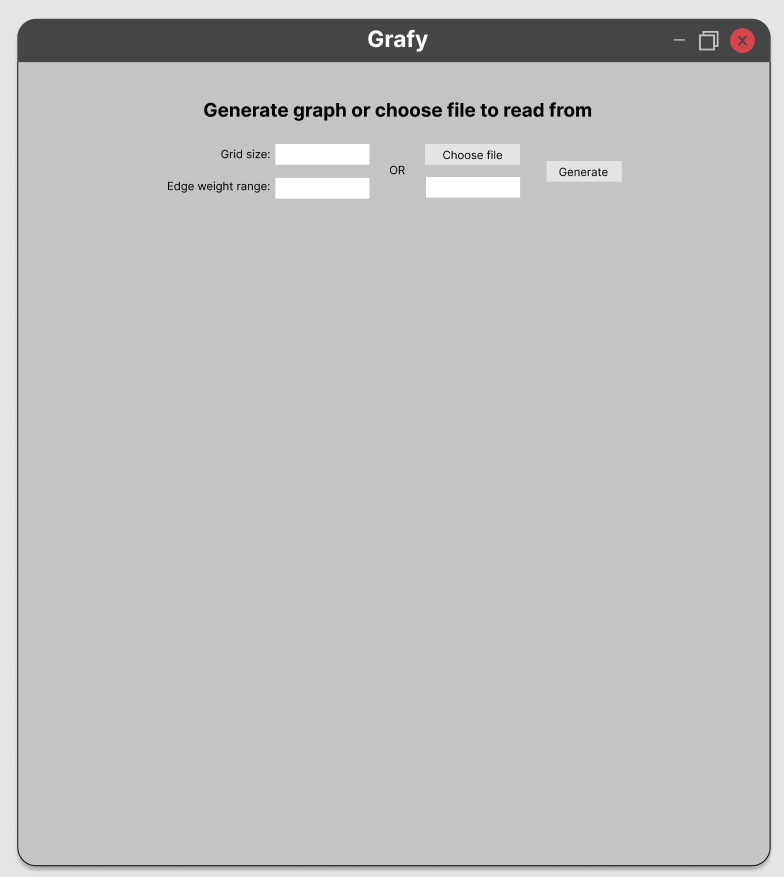
\includegraphics[height=13cm,width=10cm]{Scena_generacji_grafu.png}
\caption{Wygląd sceny generującej/wczytującej graf}
\end{figure}
\subsubsection{Wygląd sceny obsługującej graf}
\begin{figure}[h]
\centering
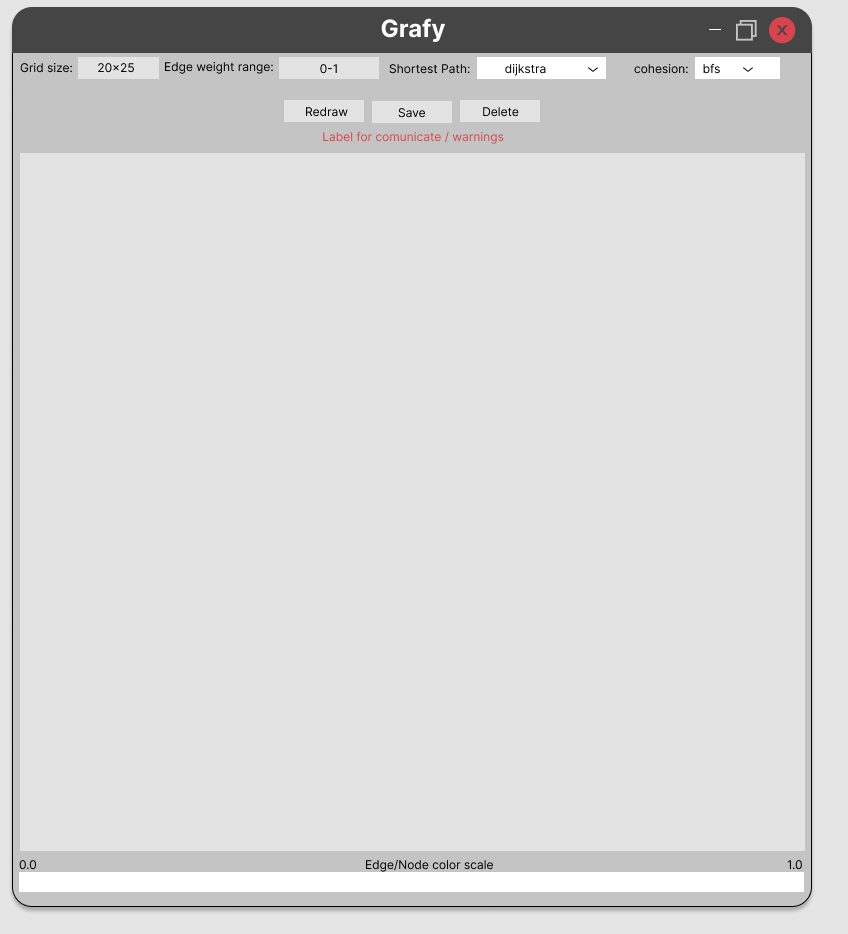
\includegraphics[height=13cm,width=10cm]{Scena_obslugujaca_graf.png}
\caption{Wygląd sceny obsługującej graf}
\end{figure}
\newpage
\subsection{Interakcje użytkownika z przyciskami, panelami i polami}
\subsubsection{Scena wczytywania grafu do programu}
W scenie, które prezentuje użytkownikowi możliwość generacji grafu lub wczytania przez użytkownika grafu z pliku. Przyciski oraz pola, które sa dostępne na scenie generowania grafu są następujące: 
\begin{itemize}
    \item \textbf{Pole tekstowe GridSize-}pole, które pozwala użytkownikowi wpisać rozmiar generowanego grafu w kratkę, biorąc pod uwagę, że użytkownik chce wygenerować graf.
    \item \textbf{Pole tekstowe Edge weight-range-}pole tekstowe, które odpowiada za odpowiedni dobór wag krawędzi w grafie. Pole tekstowe jest potrzebne do wygenerowania grafu.
    \item \textbf{Przycisk Choose File-}przycisk, który pozwala użytkownikowi wybrać plik, z którego graf w kratkę zostanie wczytany do programu.
    \item \textbf{Pole tekstowe FileName-}pole tekstowe, które odpowiada za poprawne wczytanie nazwy pliku z grafem. Jeśli użytkownik zdecyduje się wpisać nazwę ręcznie, to właśnie to pole spełnia to zadanie.
    \item \textbf{Przycisk Generate-}przycisk generate odpowiada za poprawne wygenerowanie grafu i zmianę sceny na scenę obsługującą graf w kratkę.
\end{itemize}
\subsubsection{Scena obsługująca graf}
\begin{itemize}
    \item \textbf{Pole GridSize-}pole informujące o aktualnej wielkości wczytanego grafu w kratkę.
    \item \textbf{Pole EdgeWeightRange-}pole informujące o aktualnej wielkości wygenrowanego/wczytanego grafu w kratkę.
    \item \textbf{Pole GridSize-}pole informujące o aktualnym przedziale wag krawędzi w wygenerowanym/wczytanym grafie.
    \item \textbf{Pole wyboru algorytmu najkrótszej ścieżki-}po naciśnięciu przez użytkownika przycisku wyświetla się możliwość wybrania jednego z trzech opisanych w rozdziale 3 algorytmów wyszukujących najkrótsze połączenie między wierzchołkami.
    \item \textbf{Cohesion-}po naciśnięciu przez użytkownika przycisku wyświetla się możliwość wybrania jednego z dwóch opisanych w rodziale 3 algorytmów sprawdzających spójność grafu.
    \item \textbf{Przycisk Redraw-}-przycisk po naciśnięciu usuwa znalezione najkrótsze ścieżki pomiędzy wierzchołkami, które wybrał użytkownik.
    \item \textbf{Przycisk Save-}po naciśnięciu przez użytkownika przycisku, aktualnie wczytany graf zostaje zapisany do pliku .txt mygraph.
    \item \textbf{Panel środkowy-}najważniejszy panel w programie, który odpowiada za interakcję z użytkownikiem, wyświetlanie aktualnego grafu i wyświetlanie najkrótszej ścieżki pomiędzy wybranymi przez użytkownika wierzchołkami.
    \item \textbf{Przycisk Delete-}po naciśnięciu przez użytkownika przycisku następuje powrót do sceny generującej graf, w której użytkownik od początku może wczytać/wygenerować nowy graf.
\end{itemize}
\section{Testowanie}
\subsection{Użyte narzędzia}
Testowaniem projektu zajmuje się zespół piszący cały projekt. Zadaniem testerów jest napisanie pięciu nietrywialnych i różniących się od siebie testów jednostkowych, testujących działanie programu pod kątem funkcjonalności. Zespół do przeprowadzania testów wykorzysta JUnit, dzięki której można pisać testy w czytelny sposób.
\subsection{Konwencja}
Konwencja, jaką zespół postanowił przyjąć przy pisaniu testów jednostkowych, to  wybieranie długich nazw metod, które według zespołu więcej mówią o przeprowadzanym teście. Na przykład zamiast metody testDijkstra(), zespół używa bardziej szczegółowych odniesień do testu, czyli np. shouldShowErrorDijkstraWhenNonCoherent(). Tak jak wcześniej było podkreślone, takie nazwy metod dają większa czytelność i dają programiście więcej informacji o przeprowadzanym teście.
\subsection{Warunki brzegowe}
Potencjalne błędy, które mogą wystąpić to ewentualne błędy przy generacji grafu oraz działaniu algorytmów grafowych. Zespół ma zamiar sobie z nimi poradzić następująco:
\begin{itemize}
    \item \textbf{Algorytmy wyszukujące najkrótszą ścieżkę-}napisanie testów z grafami przygotowanymi przez zespół, a następnie sprawdzenie działania wszystkich trzech algorytmów na tych grafach.Zostanie również podana weryfikacji wyświetlana na ekranie ścieżka, pokazująca najkrótszą ścieżkę.
    \item \textbf{Algorytmy badające spójność-}podobna sytuacja występuje z algorytmami badającymi spójność. Zespół przygotuje własny graf oraz sprawdzi działanie algorytmów.
\end{itemize}
\newpage
\section{Diagram klas}
Zespół zdecydował się także na wykonanie diagramu klas, który został wykonany przy pomocy Uniwersalnego Języka Modelowania(UML). Diagram klas przedstawia klasy (typy) obiektów w programie, w odróżnieniu od diagramu obiektów, który pokazuje jedynie egzemplarze (instancje) obiektów i ich zależności istniejące w konkretnym momencie. Diagram klas pokazuje zatem określony fragment struktury systemu.\\
\textbf{Wykonany przez zespół diagram klas:}
\begin{figure}[h]
\centering
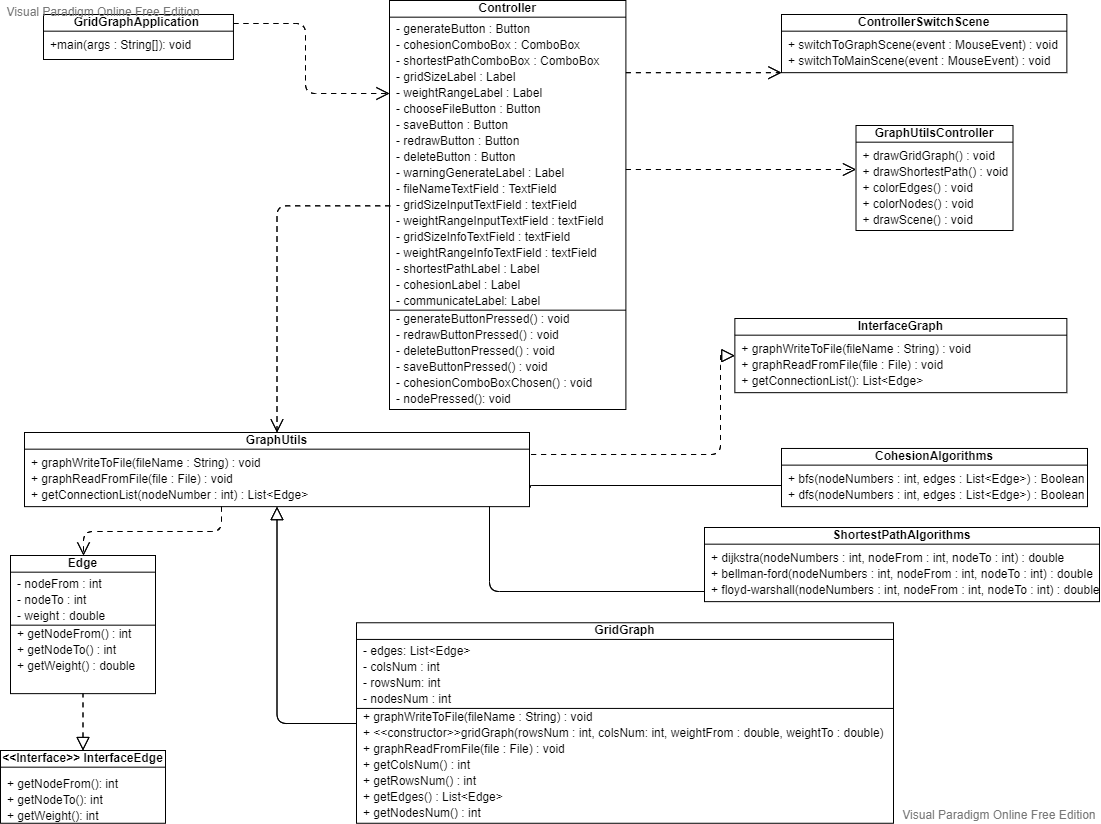
\includegraphics[height=13cm,width=13cm]{Diagram_klas_uml.png}
\caption{Diagram klas dla programu \textbf{Grafy}}
\end{figure}
\end{document}
